\chapter{Praktijktest: opstelling}
\label{appendix-c}

\section*{Teensy}

Op de Teensy microcontroller (figuur \ref{teensy-test}) wordt een microfoon aangesloten op pin A0. Het programma \texttt{TeensyAnalogRead} wordt op de Teensy uitgevoerd. Dit programma is afkomstig van het TeensyDAQ project (IPEM software). Hierdoor worden er maximum 5 analoge waarden aan een frequentie van $8000Hz$ ingelezen.

\begin{figure}[!h]
	\captionsetup{width=0.7\textwidth}
	\caption[Teensy testopstelling]{De Teensy microcontroller verbonden met een microfoon op pin A0.}
	\centering
	\advance\parskip0.3cm
	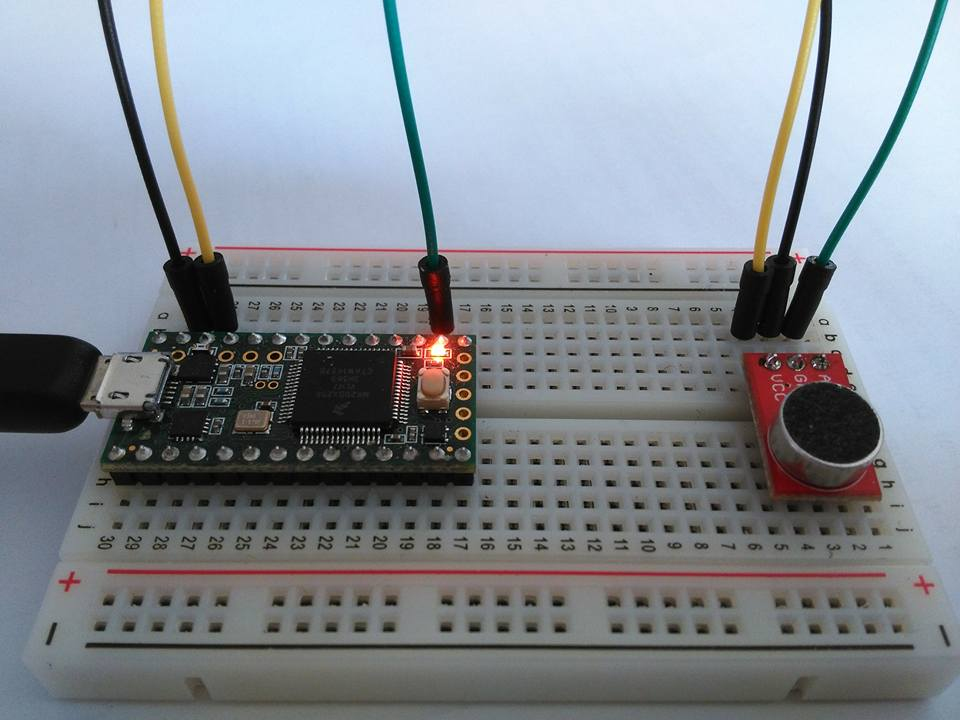
\includegraphics[width=0.4\textwidth]{teensy2.jpg}
	\label{teensy-test}
\end{figure}

\section*{Microfoon}

De andere audiostream is afkomstig van een laptopmicrofoon. Alle mogelijke verbeteringen die worden ondersteund (ruisonderdrukking en onderdrukking van akoestische echo) zijn uitgeschakeld.

\section*{Max/MSP patch}

\begin{figure}[!h]
	\captionsetup{width=0.7\textwidth}
	\caption[Max/MSP testopstelling]{De Max/MSP patch waarmee de test is uitgevoerd.}
	\centering
	\advance\parskip0.3cm
	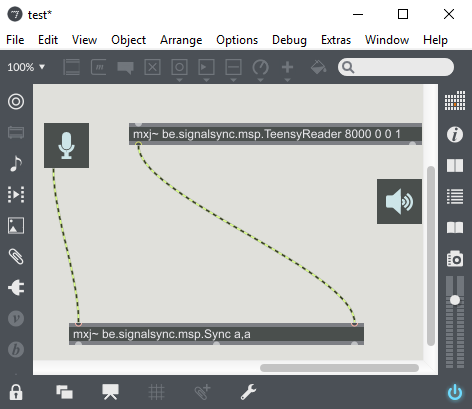
\includegraphics[width=0.6\textwidth]{maxtest.png}
	\label{max-test}
\end{figure}

De laptopmicrofoon wordt ingelezen met behulp van de \texttt{ezadc\textapprox} module. Deze module is standaard aanwezig in Max/MSP. De audiostream afkomstig van de Teensy microcontroller wordt en ingelezen met behulp van de \texttt{TeensyReader} module (geschreven voor dit onderzoek). De module is aangemaakt met volgende code:
\begin{center}
	\texttt{mxj\textapprox\ be.signalsync.msp.TeensyReader 8000 0 0 1}
\end{center}
Het synchroniseren gebeurt met de \texttt{Sync} module. Er worden geen datastreams gekoppeld aan de audiostreams. Dit is de code voor het aanmaken van de module:
\begin{center}
	\texttt{mxj\textapprox\ be.signalsync.msp.Sync a,a}
\end{center}

\section*{Resultaten}
De volgende tabel bevat de opeenvolgende gedetecteerde latencies.
\begin{table}[h!]
	\centering
	\begin{tabular}{l l|l l|l l|l l|l l}
		1 & 0.250621 & 11 & 0.249121 & 21 & 0.247121 & 31 & 0.245371 & 41 & 0.24337 \\
		2 & 0.250501 & 12 & 0.248991 & 22 & 0.247001 & 32 & 0.245121 & 42 & 0.24337 \\
		3 & 0.250371 & 13 & 0.248501 & 23 & 0.246741 & 33 & 0.244741 & 43 & 0.24299 \\
		4 & 0.250121 & 14 & 0.248251 & 24 & 0.246501 & 34 & 0.244741 & 44 & 0.24287 \\
		5 & 0.250121 & 15 & 0.248121 & 25 & 0.246241 & 35 & 0.244491 & 45 & 0.24275 \\
		6 & 0.249991 & 16 & 0.247991 & 26 & 0.246121 & 36 & 0.244491 & 46 & 0.24262 \\
		7 & 0.249621 & 17 & 0.247751 & 27 & 0.246001 & 37 & 0.244121 & 47 & 0.24262 \\
		8 & 0.249621 & 18 & 0.247491 & 28 & 0.245741 & 38 & 0.243991 & 48 & 0.24237 \\
		9 & 0.249371 & 19 & 0.247491 & 29 & 0.245501 & 39 & 0.243871 & 49 & 0.24250 \\
		10 & 0.249241 & 20 & 0.247121 & 30 & 0.245501 & 40 & 0.243751 & 50 & 0.24187 \\
	\end{tabular}
\end{table}